
\chapter{Thesis Outline}\label{ch:outline}
\section{Proposed Approach}
As discussed in the Chapter \ref{ch:lit review}, using transfer learning for designing DID is a feasible method which 
may be able to address some challenges with Arabic DID, as discussed in Sections \ref{sec:problem} and \ref{ch:background}. 
This thesis will do this through constructing different transfer learning systems and comparing their accuracy. A block diagram 
giving an overview of the system is shown in Figure \ref{fig:Block}. The portions which 
will remain consistent in the system throughout experimentation will be the initial data preprocessing which will use the python packages noisereduce 
to filter the data and perform channel normalisation. (The importance of preprocessing is covered in the section \ref{sec:dataset}.) As well as the outputting softmax layer which will classify the dialects based on the 
given categorisations. In Thesis B, the classification of 4 generalised dialects will be explored and Thesis C will look to see if the system constructed 
can then be applied to 17 regional dialects. The portions which will be investigated include the pretrained model and the downstream model. The choices for 
each have been explained in Sections \ref{sec:pretrain} and \ref{sec:tradML}. The benchmark model for each section respectively will be wav2vec 2.0 and a simple 
pooling + linear layer as the downstream model. It is expected that using XLS-R and BiLSTM will produce the system with the highest accuarcy DID. This thesis 
will also investigate the minimum amount of data required to create an effective system, to validate the claim that transfer learning is a useful method for low resource 
languages and will do this through varying both the amount of training data and the length of utterances for the test data. A breakdown of the tasks and testing which 
will be performed are in Section \ref{sec:task}. 

\begin{figure}[h!]
    \centering
    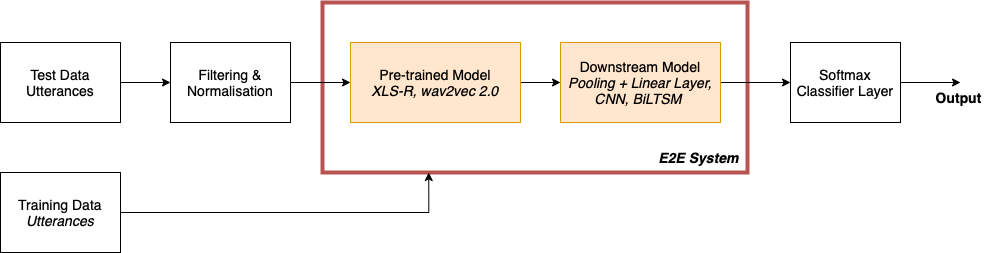
\includegraphics[width=\textwidth]{BlockDiagram.png}
    \caption{Block Diagram of Proposed Approach.}
    \label{fig:Block}
\end{figure}

\section{Expected Outcomes}
The expected outcomes of this thesis is to have designed an Arabic DID with at 
least an accuracy of 85\% for both the 4 generalised dialects and the 17 finer dialects. 
This will demonstrate that transfer learning is a viable methodology for 
creating DIDs, particularly for low resource languages and dialects.
It is also expected that using the more generalised language pretrained model XLS-R 
will outperform a model utlising wav2vec 2.0. 

\chapter{Preliminary Work}\label{ch:prelim}
During the course of Thesis A, some preliminary work was conducted to prepare for the work which will be done in 
Thesis B and Thesis C. This included gaining access to NCIS Supercomputer and setting up the SSH on my personal computer. 
Setting up the development environment with jupyter notebook, python. Downloading the training ADI17 dataset and performing 
some analysis on it which is detailed in the Section \ref{sec:dataset}. 

\section{Dataset Analysis}\label{sec:dataset}
\subsection{Dataset Selection}
There are limited dialectal Arabic datasets available, ADI17 [50], QASR [39] and the ArPod [34]
dataset were assessed as viable options to be used as training data for the DID to be designed in this 
thesis. An exploration of their features and negative characteristics is in the Table \ref{tab:dataSetChoice}.\\

\begin{table}[hbt!]
    \begin{center}
    \begin{tabular}{|m{1.5cm} || m{6cm} | m{4cm} | m{3cm}|}
        \hline
        \textbf{Dataset} & \textbf{Features} & \textbf{Associated Challenges} & \textbf{Access Status} \\
        \hline
        \hline
        ADI17 &
        {
            \textbf{Amount:} 3000hrs of\newline conversational audio on various topics.\newline
            \textbf{Source:} YouTube videos.\newline
            \textbf{Languages/Dialects:} 17 regional dialects.\newline
            Contains codeswitching. 
        }
        &
        The dataset is noisy\newline with significant amount of acoustic variation. &
        Access granted. \\
        \hline
        QASR: QCRI Aljazeera Speech Resource &
        {
            \textbf{Amount:} 2000hrs of\newline broadcast audio on various topics.\newline
            \textbf{Source:} Aljazeera broadcasting network.\newline
            \textbf{Languages/Dialects:} 3 Languages (English, French, Arabic),\newline 5 dialects (MSA, GLF, LEV,  NOR, EGY).\newline
            Contains codeswitching. 
        }&
        Even though this\newline dataset has many\newline favourable features, no contact information is provided to access the dataset.&
        Access unavailable (no contact\newline information provided)\\
        \hline
        ArPod&
        {
            \textbf{Amount:} 8hrs of high quality conversational audio.\newline
            \textbf{Source:} Podcasts.\newline
            \textbf{Languages/Dialects:} 2 Languages (English, Arabic),\newline 5 dialects (MSA, SAU, EGY, LEB, SYR).\newline
        }&
        The dataset is very small compared to alternate datasets and only contains data from a limited set of regional dialects. 
        &
        Access not\newline granted but can be obtained\newline through contacting Dr. Mourad Abbas\\
        \hline
    \end{tabular}
    \caption{Possible Dataset Choices.}
    \label{tab:dataSetChoice}
    \end{center}
\end{table}
\pagebreak
The \textbf{ADI17} dataset has been chosen to be used for this thesis as it was the most 
suitable due to a couple of reasons. Particularly it was
designed with the intention to be used for DID systems and has the largest amount of 
associated resources. 

\subsection{ADI17 Dataset}
The \textbf(ADI17) comprised of audio segments from known Youtube videos with dialects from 17 different Middle Eastern and North
African countries. The dataset is divided into training, development and test data groups. The training set contains 
3000hrs of audio total while the development and test combined is 57hrs of audio. The specifics of the dataset can be seen in Figure \ref{fig:ADI17}.
The data was collected from around 30 different Youtube channels per country and the primary dialect each Youtube channel used was verified by a human annotator. Using the Youtube channel's 
dialect audio segment's dialectal label was allocated. The training data relies on this for its labelling, whilst 
the test and development data was annotated by a human annotator. The audio segments are split into utterances, which are small portions  
of audio generated by segmenting the original audio at silence points. These silence points are usually natural pauses in conversation and a threshold 
is used to determine how long the silence must be before the audio is split. The creators of the ADI17 dataset have not specified the threshold that they used. 
The dataset is labelled using 17 regions, Thesis B explores creating a DID of 4 generalised dialects that encompass this finer set of regional dialects as shown in Figure \ref{fig:Dialectgroups}. 
So, for training in Thesis B a portion of data from each region is taken to construct the training set for the generalised dialects as shown in Figure \ref{fig:DialectSplit}. 
The core challenges with the ADI17 dataset are that the acoustics are unbalanced across each of the dialect regions and the amount of data provided is unbalanced. The amount of noise in each of the 
regions datasets is shown in Figure \ref{fig:noiseDataSet}, although its effect on the DID will be mitigated through using channel normalisation and filtering, as the papers [16, 42] have shown is effective at increasing 
accuracy of Arabic DIDs. The dataset is also unbalanced in terms of amount of training data for each region as shown in Figure \ref{fig:trainplot}, with Jordan having the least amount of data. This will not affect Thesis B, as the generalised 
dialect groups will collate portions of the data. While for Thesis C, the training data provided will be restricted to 10hrs to ensure that 
the training sets for each region are even and balanced. 


\begin{figure}[h!]
    \centering
    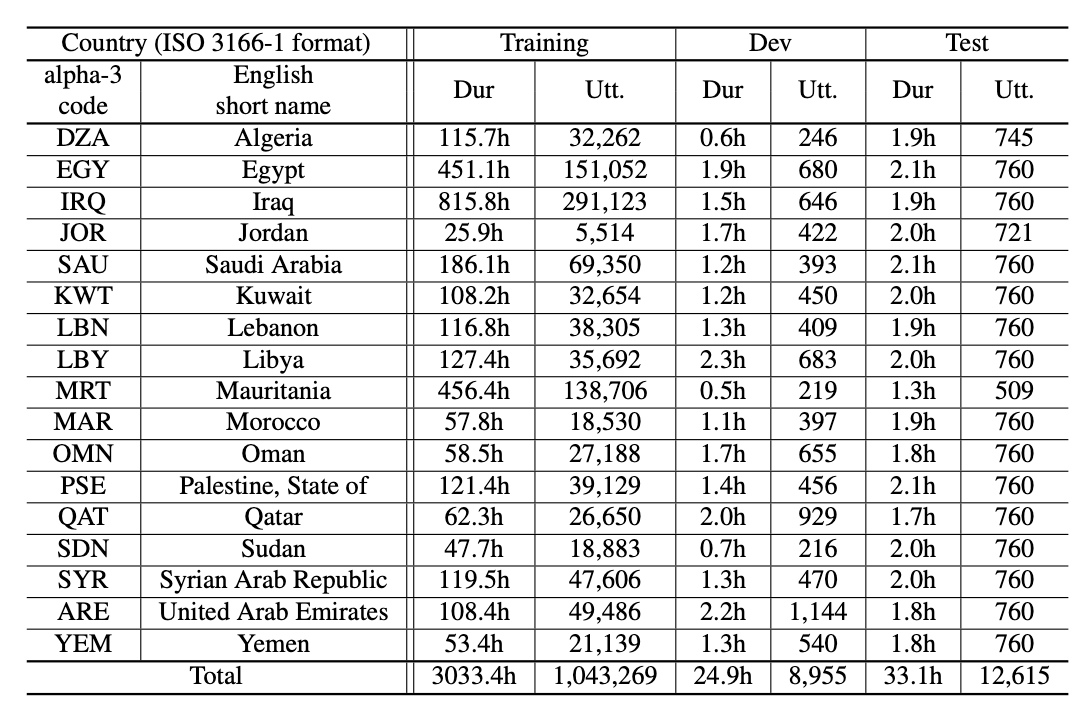
\includegraphics[width=\textwidth]{DataSetDetails.png}
    \caption{ADI17 Dataset Details.}
    \label{fig:ADI17}
\end{figure}


\begin{figure}[H]
    \CommonHeightRow{%
        \begin{floatrow}[2]%
            \ffigbox[\FBwidth]
            {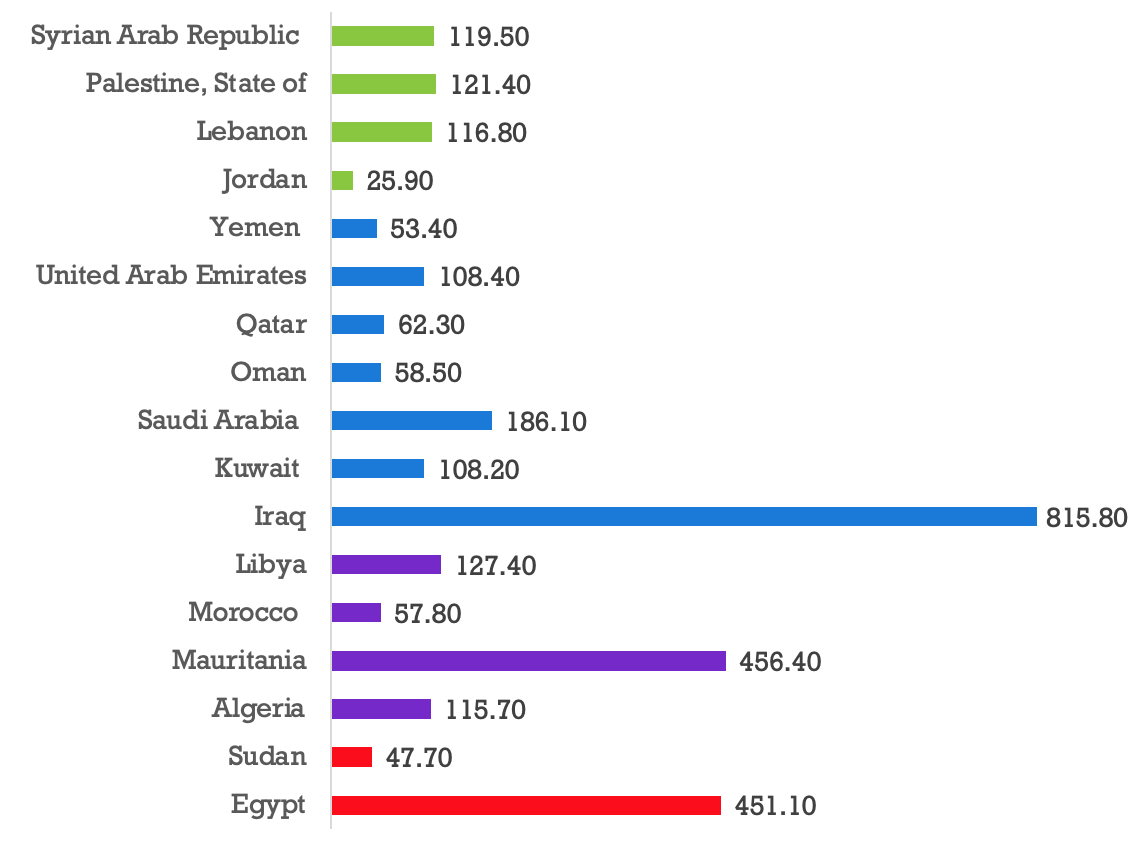
\includegraphics[height=6cm]{Trainingplot.png}}
            {\caption{Plot of ADI17 Training Data.}}\label{fig:trainplot}
            \ffigbox[\FBwidth]
            {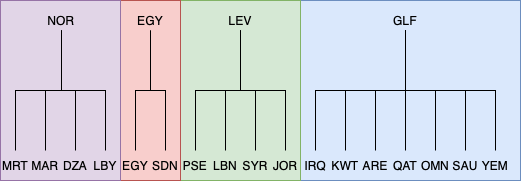
\includegraphics[height=3cm]{DialectGroups.png}}
            {\caption{ADI17 Grouped into 4 major dialects.}}\label{fig:Dialectgroups}
        \end{floatrow}}%
\end{figure}

\begin{figure}[H]
    \CommonHeightRow{%
        \begin{floatrow}[2]%
            \ffigbox[\FBwidth]
            {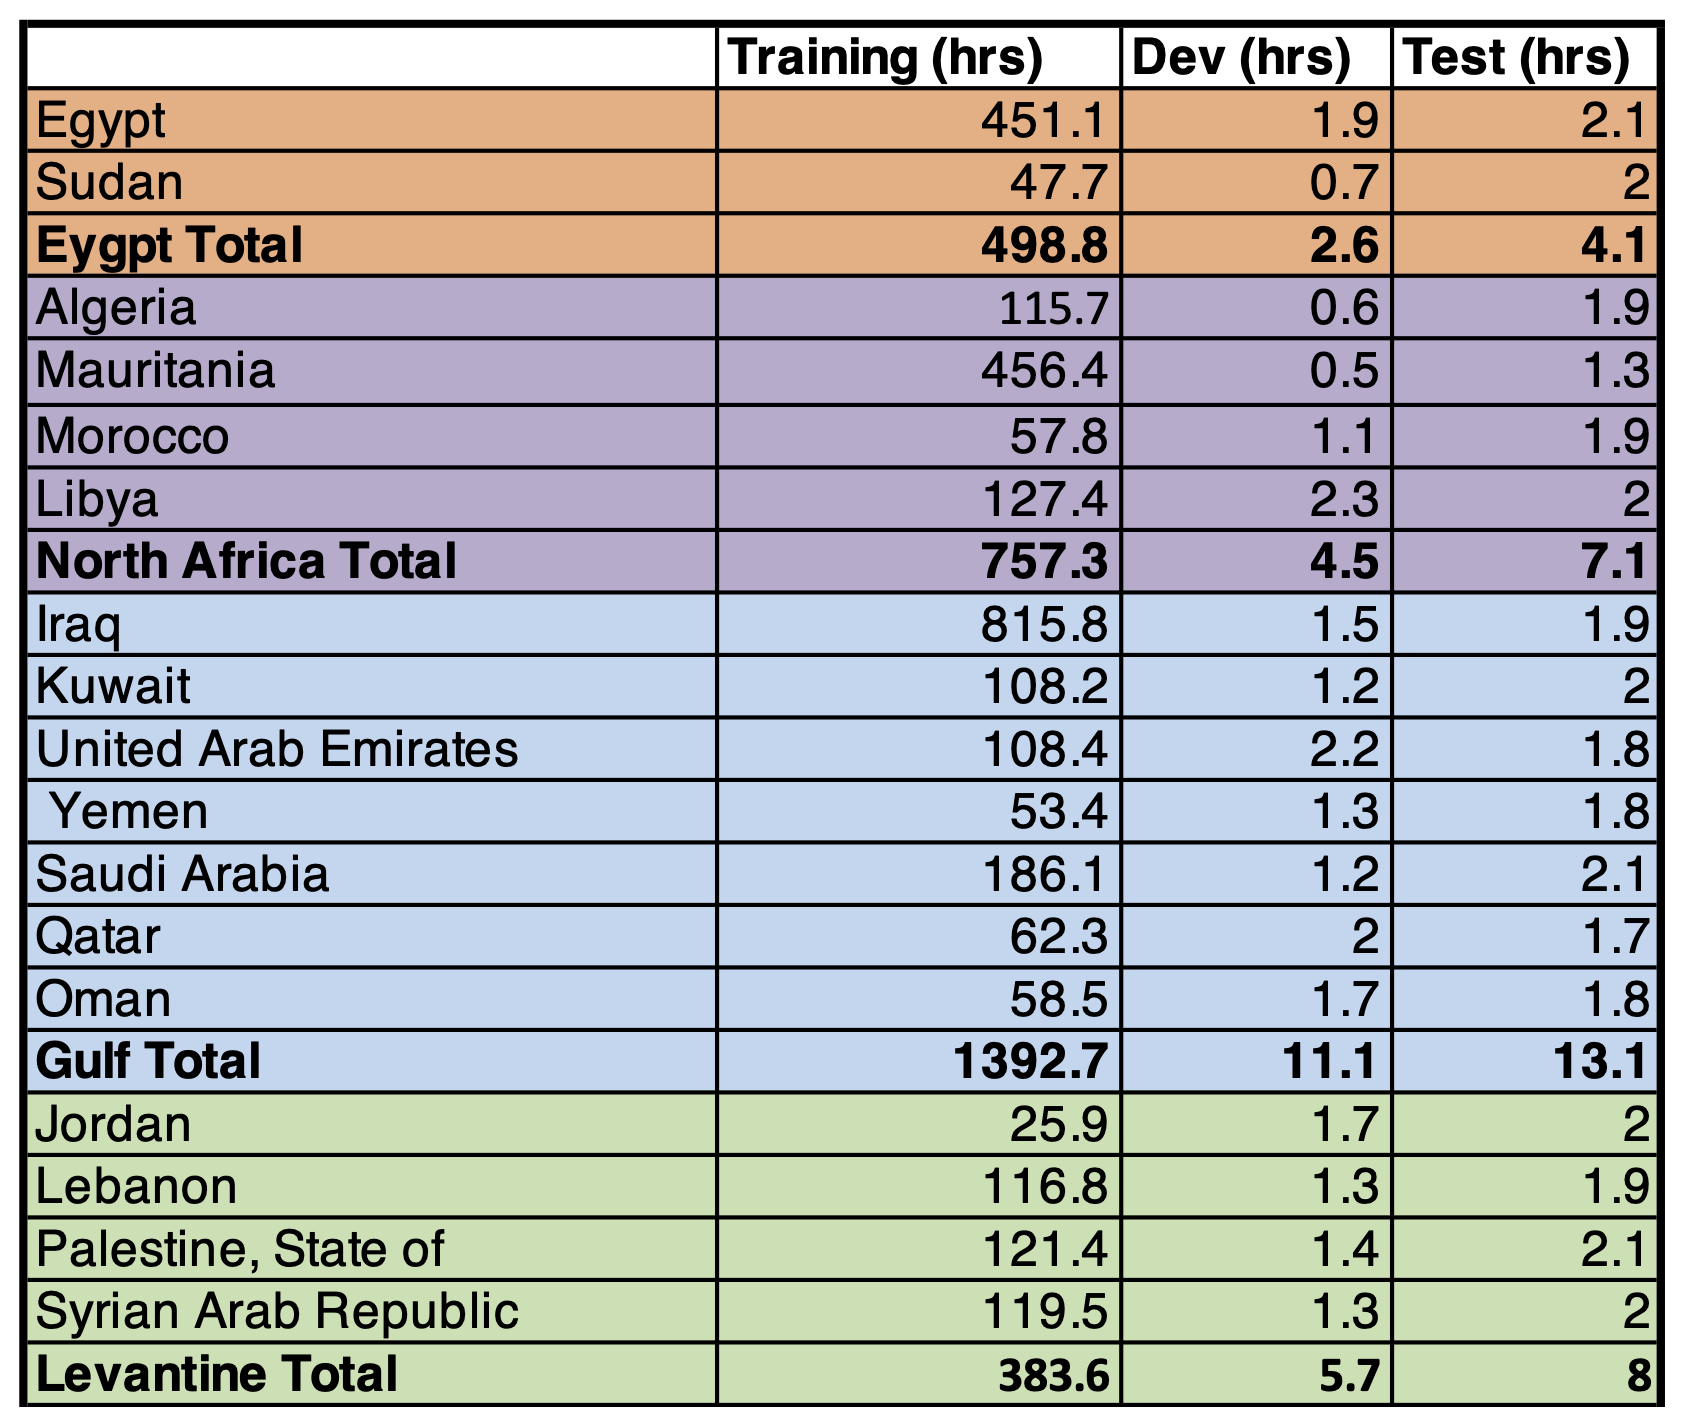
\includegraphics[height=7cm]{ADI17_Dataset.png}}
            {\caption{Total data for each of the 4 dialects.}}\label{fig:DialectAmount}
            \ffigbox[\FBwidth]
            {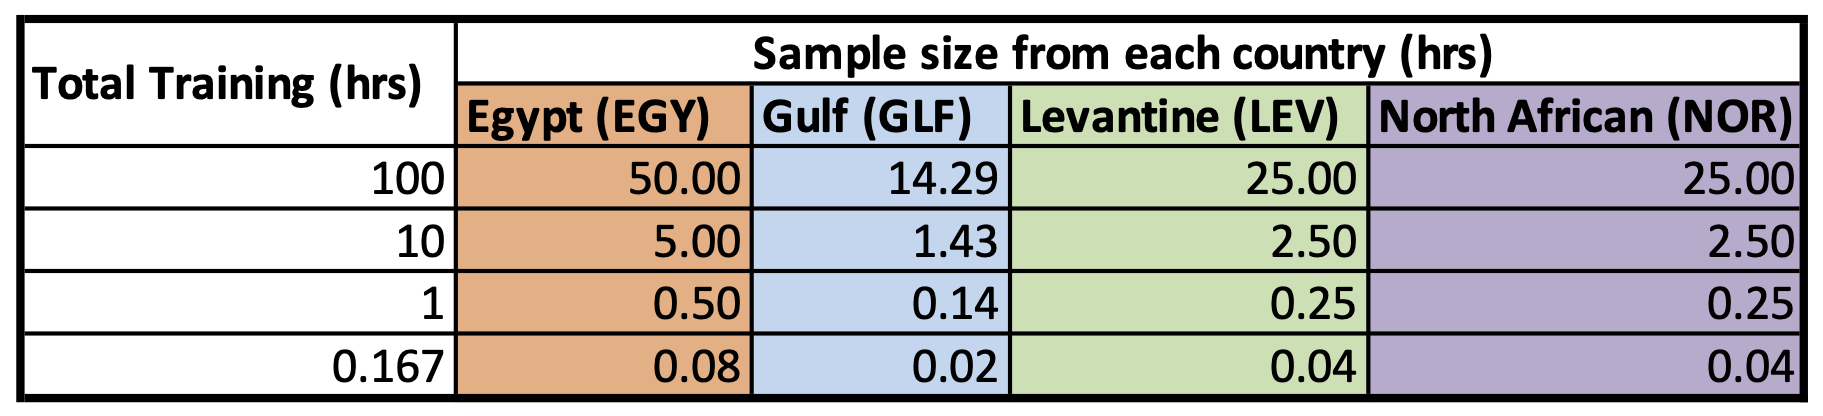
\includegraphics[height=2cm]{ADI17_split.png}}
            {\caption{ADI17 Grouped into 4 dialect groups.}}\label{fig:DialectSplit}
        \end{floatrow}}%
\end{figure}

\begin{figure}[h!]
    \centering
    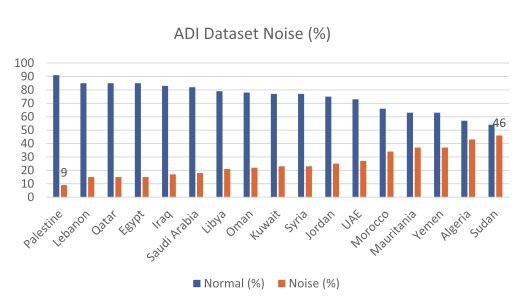
\includegraphics[width=\textwidth]{noiseDataset.png}
    \caption{ADI17 Dataset Noise levels. [6]}
    \label{fig:noiseDataSet}
\end{figure}





\chapter{Thesis Plan}\label{ch:plan}
\section{Timeline Overview}
An overview of summarising the planned timeline for this thesis is presented in 
Figure \ref{Gantt Chart}. Tasks have been broken into manageable 2-3 week intervals and testing, evaluating
and assignment preparation have also been accounted for in the timeline. 
Thesis A has comprised mainly of finding a focus topic, developing a sound understanding of the background information on dialectal Arabic, 
LIDs, DIDs and transfer learning. Evaluated possible datasets, prebuilt models, python packages and downstream models 
to be implemented in Thesis B. As well as gaining access to the Gadi supercomputer, dataset and performing some data analysis on the set. 

The majority of the implementation and experimentation for this thesis will occur in 
Thesis B. The dataset preprocessed using python audio processing packages such as NoiseReduce and PyAudio. 
The main machine learning model with the pretrained model and downstream model will be implemented
using the SpeechBrain Python toolkit.

Thesis C focus will focus on evaluating the performance of the model developed in Thesis B and further 
developing it. This evaluation will be done through changing the amount of classifier groups from 4 to 17. 
In addition to testing the model with various utterance lengths. There has been significant time allocated in 
Thesis C for reflecting, testing and iterating upon the model designed. 

\begin{figure}[h]
    \centering
    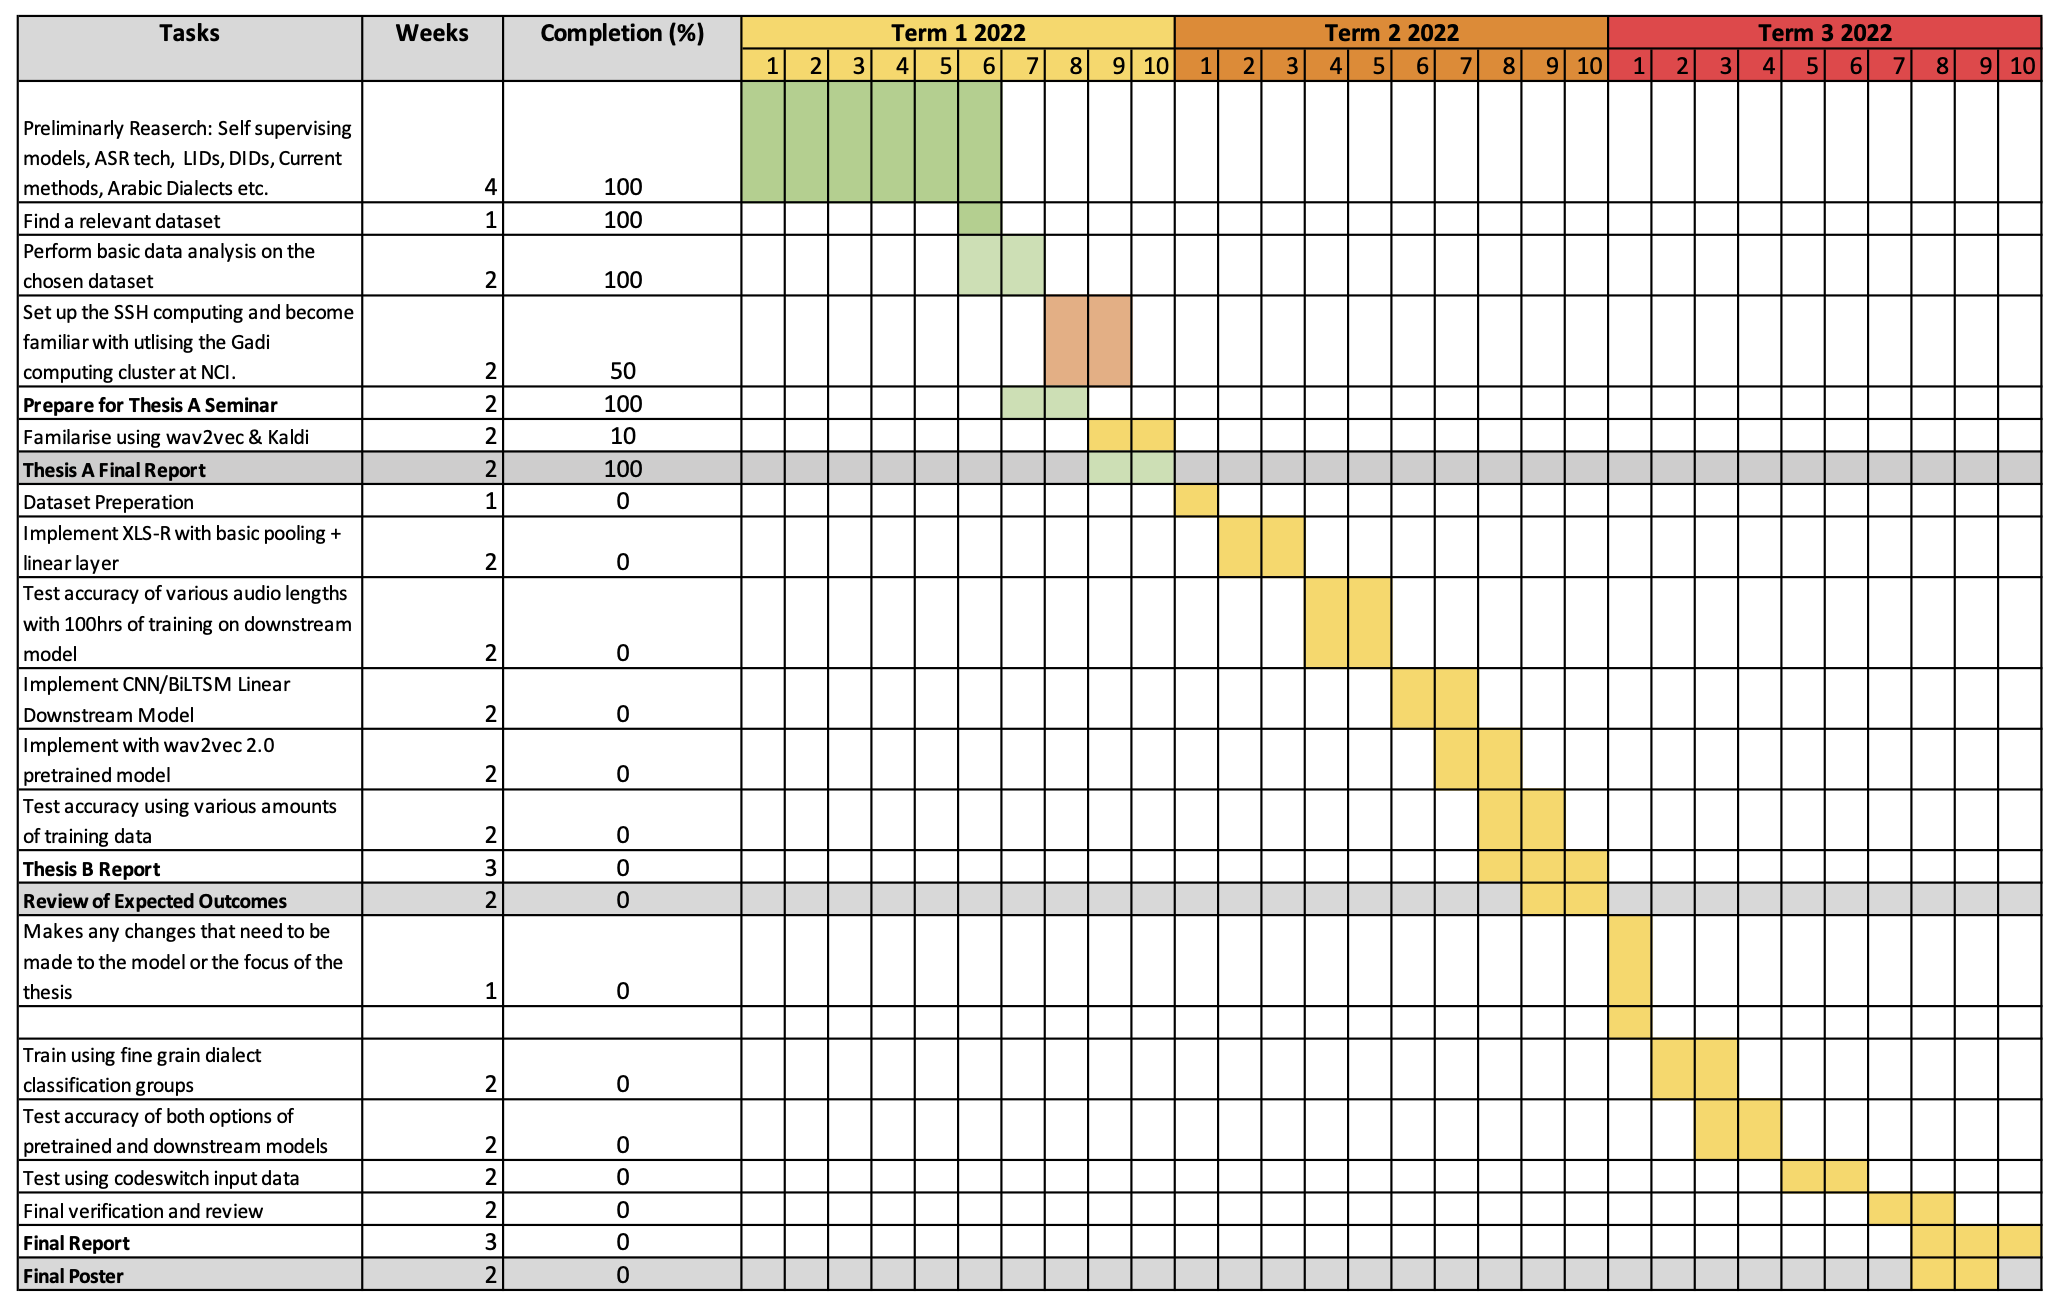
\includegraphics[width=\textwidth]{images/timeline.png}
    \caption{Gantt Chart.}\label{Gantt Chart}
\end{figure}
\section{Thesis B}
\subsection{Aims}
Thesis B will investigate various methods for designing a DID for the 4 major
Arabic dialects (EGY, GLF, LEV, NOR). All testing done in Thesis B will be done with 
120sec utterance test data.\\
The goals of Thesis B are as follows: 
\begin{itemize}
    \item Investigate the system's performance and determine if it is robust for low resource dialects. 
    \item Benchmark a generalised language pretrained model against an English speech pretrained model.
    \item Determine the most accurate downstream model architecture. 
\end{itemize}

\subsection{Task Breakdown}\label{sec:task}

\begin{enumerate}
    \item Dataset preprocessing. 
    \item Build basic model (XLS-R, Linear Layer + Pooling).
    \item Determine the minimum amount of labelled data required through training with:
    \begin{itemize}
        \item 100hrs
        \item 10hrs 
        \item 1hr 
        \item 10mins
    \end{itemize} 
    \item Benchmark against wav2vec 2.0. 
    \item Build model with CNN downstream architecture. 
    \begin{itemize}
        \item XLS-R with labelled data: 
        \begin{itemize}
            \item 100hrs
            \item 10hrs 
            \item 1hr 
            \item 10mins
        \end{itemize} 
        \item wav2vec 2.0 with labelled data: 
        \begin{itemize}
            \item 100hrs
            \item 10hrs 
            \item 1hr 
            \item 10mins
        \end{itemize} 
    \end{itemize}
    \item Build model with BiLSTM downstream architecture.
    \begin{itemize}
        \item XLS-R trained with labelled data: 
        \begin{itemize}
            \item 100hrs
            \item 10hrs 
            \item 1hr 
            \item 10mins
        \end{itemize} 
        \item wav2vec 2.0 with labelled data: 
        \begin{itemize}
            \item 100hrs
            \item 10hrs 
            \item 1hr 
            \item 10mins
        \end{itemize} 
        \item Experiment fine tuning with unlabeled data
    \end{itemize}
\end{enumerate}

\section{Thesis C}
\subsection{Aims}
Thesis C will extend upon the conclusions found in Thesis B, assessing the robustness and performance of 
the DID designed through using a finer set of 17 dialect classifications 
(DZA, EGY, IRQ, JOR, SAU, KWT, LBN, LBY, MRT, MAR, OMN, PSE, QAT, SDN, SYR, ARE, YEM).\\
The goals of Thesis C are as follows: 
\begin{itemize}
    \item Prove a model can be used to identify a finer set of dialectal groups 
    \item Evaluate the performance of the DID with utterances of various lengths.  
\end{itemize}
\subsection{Task Breakdown}

\begin{enumerate}
\item Assess the most accurate model from Thesis B and adapt it to include the 17 classifier groups.
\item Observe its accuracy with labelled training data:
    \begin{itemize}
        \item 10hrs 
        \item 1hr 
        \item 10mins
    \end{itemize}
\item Evaluate the DID's accuracy with utterances of:
    \begin{itemize}
        \item 10hrs 
        \item 1hr 
        \item 10mins
    \end{itemize}
\end{enumerate}


\section{Possible Challenges}
The major challenges likely to be encountered in this thesis are:\\
\textbf{Quality of Dataset:} There is acoustic variation across the dataset such as environmental noise and variation in the volume. 
The acoustic variation could lead to the network overfitting and classifying based upon acoustic rather than linguistic dialectal differences. 
As a non-Arabic speaker, I will be unable to audibly verify the accuracy of the dataset or identify any mislabeling errors.
Filtering will be used to mitigate the acoustic variation within the dataset and 
since, multiple papers have utlised the ADI17 dataset there is confidence that the dataset is reliable.\\\\
\textbf{Time:} Machine learning systems especially when training with large amounts of data (100hrs) take time to process. So, tuning metaparameters 
and making design changes may take several hours to present results. This time delay will make debugging challenging, 
although by anticipating for this time delay and staying organised the effect this will have can be reduced. \\\\
\textbf{Tuning Metaparamaters:}
There are various different metaparameters, pruning methods and optimisers which can be used in designing a machine learning model. Tuning these will 
take a significant amount of time, writing a script to cycle through different metaparameters can increase the efficiency of this task.\\\\
\textbf{Negative Transfer:} In transfer learning, there is the risk that previous knowledge of a pretrained model may 
damage the performance of specific task. This may cause significant issues so, by testing multiple amounts of training data and models, the occurance of  
negative transference can be assessed. [62]